\documentclass{article}
\usepackage[utf8]{ctex}
\usepackage{tabularray}
\usepackage{graphicx}
\usepackage{float}
\usepackage{indentfirst}
\usepackage{geometry}
\usepackage[table,xcdraw]{xcolor}
\usepackage{longtable}
\usepackage{adjustbox}
\newcommand{\enabstractname}{Abstract}
\newcommand{\cnabstractname}{摘要}
\newenvironment{enabstract}{%
  \par\small
  \noindent\mbox{}\hfill{\bfseries \enabstractname}\hfill\mbox{}\par
  \vskip 2.5ex}{\par\vskip 2.5ex}
\newenvironment{cnabstract}{%
  \par\small
  \noindent\mbox{}\hfill{\bfseries \cnabstractname}\hfill\mbox{}\par
  \vskip 2.5ex}{\par\vskip 2.5ex}
  
\usepackage{listings}
  \lstset{
language=verilog,                        % Code language
basicstyle=\small\ttfamily,             % Code font, Examples: \footnotesize, \ttfamily
keywordstyle=\color{purple},            % Keywords font ('*' = uppercase)
commentstyle=\em\color{gray},           % Comments font
numbers=left,                           % Line nums position
numberstyle=\tiny\ttfamily,             % Line-numbers fonts
stringstyle=\color{mauve},
stepnumber=1,                           % Step between two line-numbers
numbersep=5pt,                          % How far are line-numbers from the code
frame=single,                               % A frame around the code
aboveskip=3mm,
belowskip=3mm,
tabsize=4,                              % Default tab size
captionpos=b,                           % Caption-position = bottom
breaklines=true,                        % Automatic line breaking?
breakatwhitespace=false,                % Automatic breaks only at white space?
showspaces=false,                       % Don't make spaces visible
showstringspaces=false,
showtabs=false,                         % Don't make tables visible
basewidth=0.5em,
morekeywords={True, False},
columns=flexible,
keepspaces=true
}


\setlength{\parindent}{2em}
\geometry{a4paper,scale=0.7}

\title{
\begin{large}
操作系统课程设计\\
\end{large}
Project3: File System
}

\author{周旭东 521021910829}
\date{2023.05.23}

\begin{document}

\maketitle

\begin{cnabstract}

在 Project3 中,首先设计和实现了一个基本的类似磁盘的辅助存储服务器;接着实现了一个基本的 FAT 结构文件系统;在此基础上用磁盘当服务器,用 socket 套接字使得文件系统能够和磁盘服务器交互写作,形成一个非易失文件系统,并将其作为第二级服务器,用客户端连接访问。 并在 linux 系统上进行了测试。

\end{cnabstract}


\tableofcontents
\newpage

\section{Step1: Design a basic disk-storage system}

实现物理磁盘的模拟。模拟磁盘按柱面和扇区进行组织,并考虑轨道到轨道的时间。(使用usleep(3C),nanosleep(3R)等)。以微秒为单位的值(可能不是整数),作为命令行参数传递给磁盘存储系统。此外,让柱面数和每个柱面的扇区数作为命令行参数。扇区大小固定为 256 字节。将此文件的文件名作为另一个命令行选项。

\subsection{实现要点}

\subsubsection{存储映射}

首先,使用open函数打开指定的文件filename,使用O\_RDWR标志表示以可读可写的方式打开文件,O\_CREAT标志表示如果文件不存在则创建它,S\_IRUSR | S\_IWUSR表示设置文件权限为用户可读可写。

接下来,使用lseek函数将文件指针移动到文件末尾前一个字节的位置。这样做是为了“扩展”文件大小,确保映射的内存空间足够容纳整个文件。

然后,代码使用write函数向文件写入一个空字节,以实际改变文件大小。

\begin{lstlisting}
	// Open disk file and map it into memory
    fd = open(filename, O_RDWR | O_CREAT, S_IRUSR | S_IWUSR);
    if (fd == -1) {
        printf("Error: Could not open file '%s'.\n", filename);
        exit(-1);
    }
    if (lseek(fd, FILESIZE - 1, SEEK_SET) == -1) {
        printf("Error calling lseek() to 'stretch' the file\n");
        exit(-1);
    }
    if (write(fd, "", 1) == -1) {
        printf("Error writing last byte of the file\n");
        exit(-1);
    }
\end{lstlisting}

使用mmap函数将文件映射到内存中。参数NULL表示由系统选择合适的映射地址,FILESIZE指定映射的长度为文件大小,PROT\_READ | PROT\_WRITE表示内存区域可读可写,MAP\_SHARED表示对映射区的修改对其他映射同一文件的进程可见,fd是打开的文件描述符,0表示映射起始位置相对于文件开头的偏移量。

\begin{lstlisting}
	disk_data = mmap(NULL, FILESIZE, PROT_READ | PROT_WRITE, MAP_SHARED, fd, 0);
	if (disk_data == MAP_FAILED) {
        close(fd);
        printf("Error:Could not map file.\n");
        exit(-1);
    }
\end{lstlisting}

在处理完所有指令后,解除文件的内存映射并关闭相关的文件描述符。

\begin{lstlisting}
	// Unmap and close
    if (disk_data != NULL && munmap(disk_data, FILESIZE) == -1) {
        perror("munmap");
        return -1;
    }
    if (fd != -1 && close(fd) == -1) {
        perror("close");
        return -1;
    }
    close(fd_log);
\end{lstlisting}

\subsubsection{指令处理}

依照要求,需要支持的指令有:

\begin{itemize}
	\item I:信息请求。磁盘返回两个表示磁盘几何的整数:柱面数和每个柱面的扇区数。
	\item R c s:对柱面 c 扇区 s 的内容的读取请求。磁盘返回 Yes,后跟写空间和这 256 字节的信息,如果不存在此类块,则返回 No。
	\item W c s data:编写圆柱体 c 扇区 s 的请求。磁盘返回 Yes 并将数据写入柱面 c 扇区 s(如果是有效的写入请求)或返回 No。
	\item E:退出磁盘存储系统。
\end{itemize}

在一个循环中持续支持指令,直到读取到“E”,将 break 出循环体。用 scanf 对输入的字符串进行解析,并做扇区越界判断。符合要求时进行磁盘操作,所操作位置为

 \verb| disk_data + (c * SECTORS + s) * BLOCKSIZE|
 
 并使用 usleep 函数根据两次读写位置的差值进行磁盘读写的延迟模拟。
 
  \verb| usleep(track_to_track_time * abs(c - last_c));|

\begin{lstlisting}
while (1) {
        scanf("%c", &cmd);
        if (cmd == 'E') {
            // Exit
            printf("Goodbye!\n");
            break;
        }
        else if (cmd == 'I') {
            // Information request
            printf("%d %d\n", CYLINDERS, SECTORS);
        } 
        else if (cmd == 'R') {
            // Read request
            scanf("%d %d", &c, &s);
            if (c < 0 || c >= CYLINDERS || s < 0 || s >= SECTORS) {
                printf("No\n");
            } 
            else {
                printf("Yes ");
                memcpy(data, disk_data + (c * SECTORS + s) * BLOCKSIZE, BLOCKSIZE);
                fwrite(data, sizeof(char), strlen(data), stdout);
                printf("\n");
                usleep(track_to_track_time * abs(c - last_c));
            }
        }
        else if (cmd == 'W') {
            // Write request
            scanf("%d %d", &c, &s);
            if (c < 0 || c >= CYLINDERS || s < 0 || s >= SECTORS) {
                printf("No\n");
            }
            else {
                fgets(data, BLOCKSIZE, stdin);
                memcpy(disk_data + (c * SECTORS + s) * BLOCKSIZE, data, strlen(data)-1);
                printf("Yes\n");
                usleep(track_to_track_time * abs(c - last_c));
            }
        }
        else if(cmd == '\n')continue;
        else {
            printf("Instructions Error!\n");
        }
        last_c = c;
    }
\end{lstlisting}

\subsubsection{日志维护}

由于前期调试的需要,将所有信息使用 printf 直接输出到标准输出流,为转而进行日志记录,使用 dup2 重定向输出流到日志中。在此之前需要设置日志文件:使用open函数打开名为"disk.log"的文件。使用参数O\_WRONLY表示以只写方式打开文件,O\_CREAT表示如果文件不存在则创建它,S\_IRUSR | S\_IWUSR表示设置文件权限为用户可读可写。

\begin{lstlisting}
	int fd_log = open("disk.log", O_WRONLY | O_CREAT, S_IRUSR | S_IWUSR);
    if (fd_log == -1) {
        perror("Error: Could not open file 'disk.log'.\n");
        exit(-1);
    }
    // redirect using dup2
    if (dup2(fd_log, STDOUT_FILENO) == -1) {
        perror("Error: Could not dup.");
        exit(-1);
    }
\end{lstlisting}

\subsection{功能测试}

\begin{figure}[H]
\center
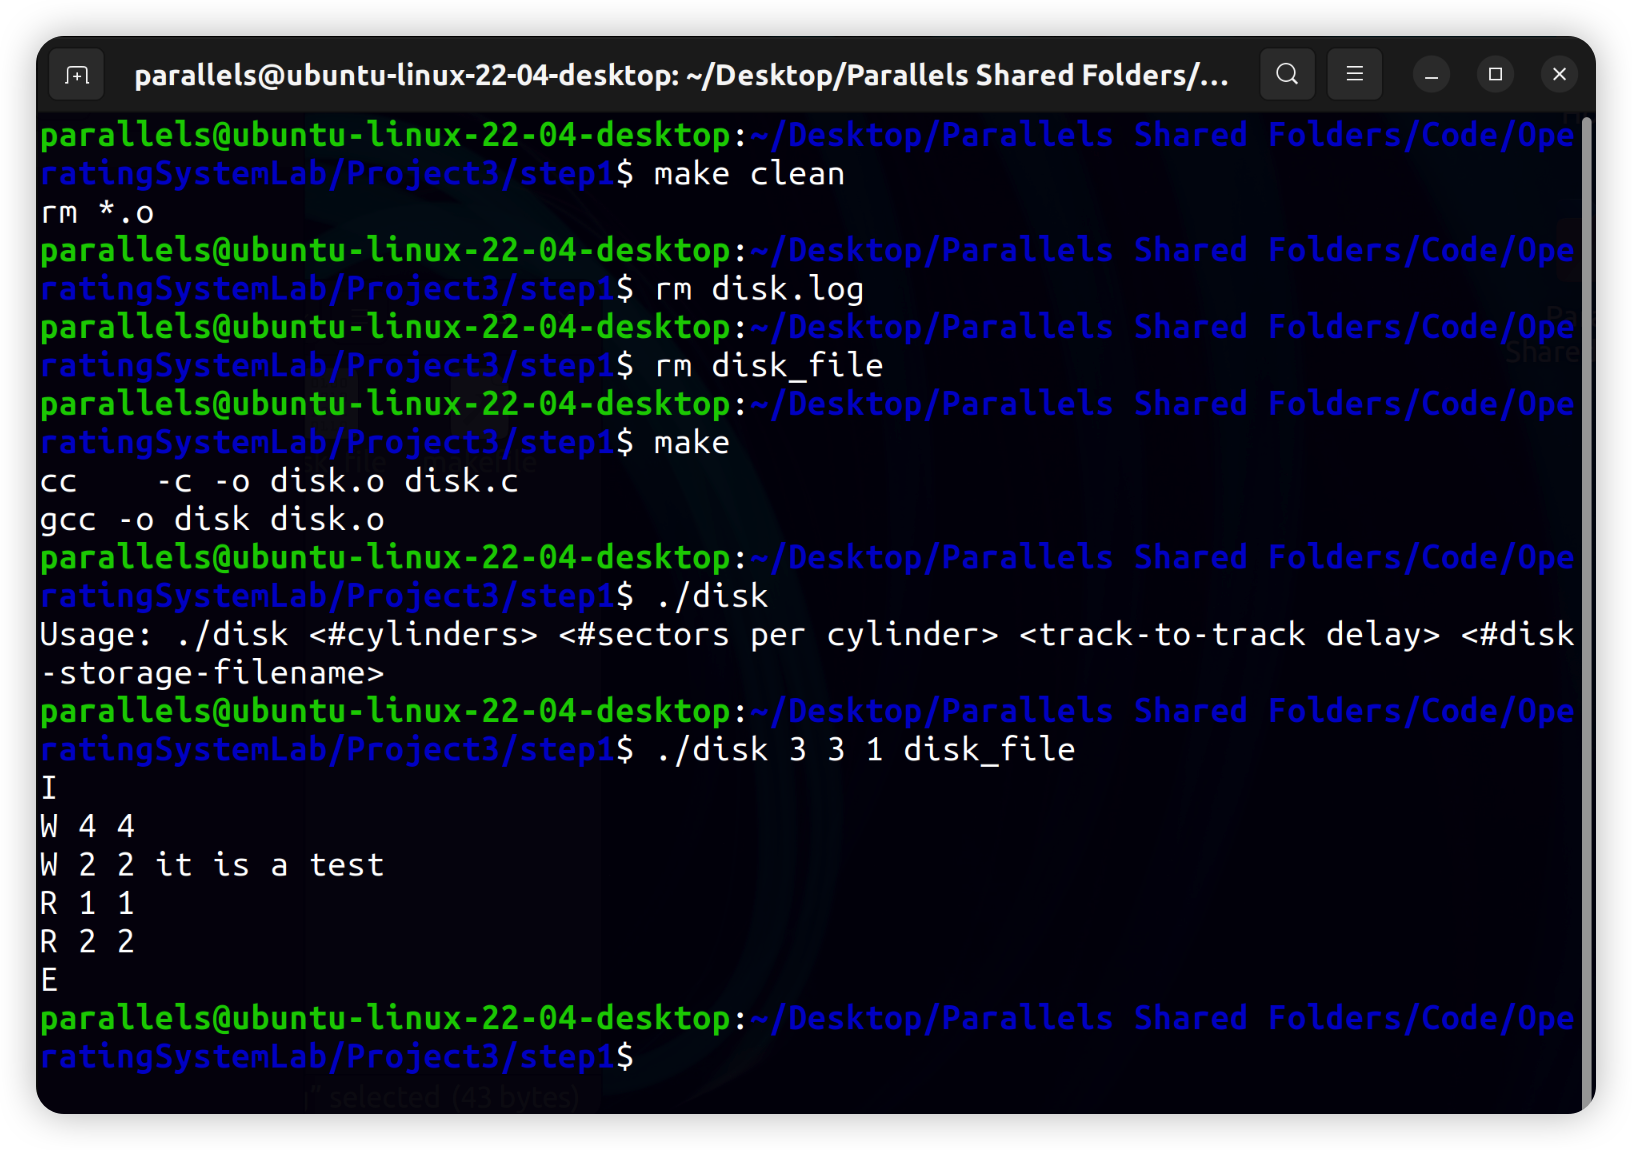
\includegraphics[scale = 0.45]{s1-t1.png}
\caption{Step1测试}
\label{s1-t1}
\end{figure}

如图\ref{s1-t1}进行测试,顺序为:用 I 读取磁盘信息,写越界位置,写正常位置内容,读空白位置,读刚写入的位置,退出。

日志内容如图\ref{s1-t2}所示,结果符合要求。

\begin{figure}[H]
\center
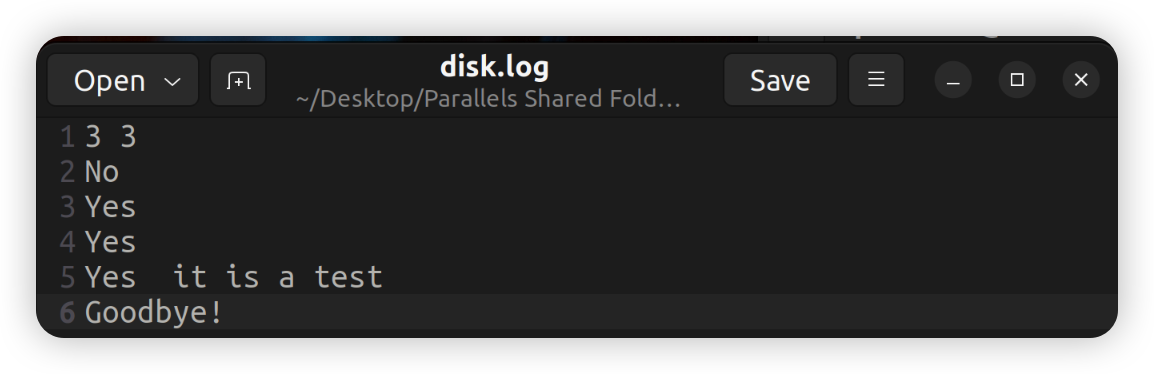
\includegraphics[scale = 0.65]{s1-t2.png}
\caption{Step1测试}
\label{s1-t2}
\end{figure}

%\begin{lstlisting}
%	printf("hello\n");
%\end{lstlisting}

\section{Step2: Design a basic file system}

\subsection{实现要点}

\subsubsection{FAT系统基础构建}

文件系统构建思路为将目录和文件都看作 file存储,以 type 进行辨别,好处是在后期与物理磁盘交互时打包数据块更为方便简洁。

目录项包含了文件的相关信息。其结构如图\ref{s2-1}所示。

\begin{figure}[H]
\center
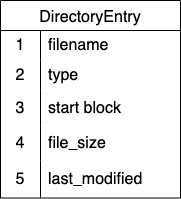
\includegraphics[scale = 0.6]{s2-1.png}
\caption{目录项结构}
\label{s2-1}
\end{figure}

filename:文件名。数组的大小为文件名的最大长度。type:表示文件类型。取值为“F","D",表示普通文件或目录。start\_block:一个整数,表示文件起始块的位置或索引。它指示文件在存储介质(例如磁盘)上的起始位置。file\_size:文件的大小。last\_modified:文件的最后修改时间。

\verb| root_directory[MAX_FILE_ENTRIES] |是目录项的实例化。

\verb| char disk[NUM_BLOCKS][BLOCK_SIZE]; |为构建的虚拟磁盘,存储每个文件的相应内容,大小为 [BLOCK\_SIZE]

\begin{lstlisting}
// DirectoryEntry struct
typedef struct {
    char filename[MAX_FILENAME_LENGTH];
    char type;
    int start_block;
    int file_size;
    char* last_modified;
} DirectoryEntry;

DirectoryEntry root_directory[MAX_FILE_ENTRIES];
char disk[NUM_BLOCKS][BLOCK_SIZE];
\end{lstlisting}

由于每个文件大小不做要求,假定都为 256bytes 以内,将 StartBlock 作为文件分配的唯一数据块,给出此系统的结构示意图\ref{s2-2}

\begin{figure}[H]
\center
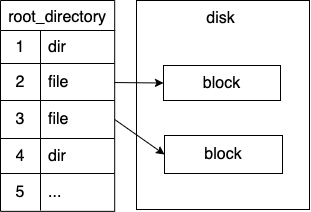
\includegraphics[scale = 0.6]{s2-2.png}
\caption{目录和文件块分配}
\label{s2-2}
\end{figure}

另外,针对目录项和虚拟磁盘,给出两个函数用于在给定的数据结构中查找空闲的目录项和空闲的数据块。以方便文件的创建和删除等操作。

\begin{lstlisting}
int find_free_entry() {
    for (int i = 0; i < MAX_FILE_ENTRIES; i++) {
        if (root_directory[i].filename[0] == '\0')
            return i;
    }
    return -1;
}

int find_free_block() {
    for (int i = 0; i < NUM_BLOCKS; i++) {
        if (disk[i][0] == '\0')
            return i;
    }
    return -1;
}
\end{lstlisting}

\subsubsection{指令处理}

根据指令要求给出实现函数。

\noindent\textbf{f:格式化。这将通过初始化文件系统所依赖的任何/所有表来格式化磁盘上的文件系统。}

将所有的数据块和目录项 table 用空字符串替换,即格式化整个文件系统。

\begin{lstlisting}
void clear_all() {
    for(int i = 0; i < MAX_FILE_ENTRIES; i++){
        strcpy(root_directory[i].filename, "");
        if(root_directory[i].type == 'F')
            strcpy(disk[root_directory[i].start_block], "\0");
        root_directory[i].file_size = 0;
    }
    printf("Done\n");
}
\end{lstlisting}

\noindent\textbf{mk f : 创建文件。这将在文件系统中创建一个名为 f 的文件。\\ 
mkdir d:创建目录。这将在当前目录中创建一个名为 d 的子目录。}

create\_file函数负责创建文件,并将文件名、类型、起始块位置、文件大小和最后修改时间等信息存储到文件系统的目录中。寻找到空白目录项之后,对所创建的文件类型分情况,若为目录,则不分配数据块,若为文件则分配一个 block 大小的数据块并用 tab 占位防止后续查找空余块时发生重合。

在创建文件时用 time 函数设置时间并用 ctime 转为字符串后保存到 last\_modified 中。需要注意的是,这里的时间末尾带有一个换行符,使用字符串操作手动去除。

此外需定义全局变量\verb|char current_directory[MAX_PATH_LENGTH] = "/";|,每次启动文件系统初始化当前目录为 /。使用该变量作为查找文件和设置文件名称。文件命名时会带上当前目录,方便查找和后续目录切换功能。

例如,位于 /test 目录下的文件 /main.c 的名称为 /test/main.c

\begin{lstlisting}
void create_file(const char* name, char type) {
    char* filename= concat_strings(current_directory, name);
    if(find_file(name) != -1){
        free(filename);
        return;
    } 
    int entry_index = find_free_entry();
    if (entry_index == -1) {
        printf("No: full\n");
        free(filename);
        return;
    }

    strcpy(root_directory[entry_index].filename, filename);
    root_directory[entry_index].type = type;
    if(type == 'D'){
        root_directory[entry_index].start_block = 0;
        root_directory[entry_index].file_size = 0;
    }
    else{
        root_directory[entry_index].start_block = find_free_block();
        strcpy(disk[root_directory[entry_index].start_block], "0");
        root_directory[entry_index].file_size = 1;
    }

    printf("Yes\n");
    // set last modified time
    time_t current_time;
    time(&current_time);
    root_directory[entry_index].last_modified = ctime(&current_time);
    root_directory[entry_index].last_modified[strlen(root_directory[entry_index].last_modified) - 1] = '\0';
    
    free(filename);
}
\end{lstlisting}

\noindent\textbf{cd path:更改目录。这会将当前工作目录更改为路径,初始工作路径为 /。需要处理 cd . 和 cd .. 。}

切换目录在该文件系统下为字符串操作,cd.. 进入上一目录时用 strrchr 读取上一个 / 以内的内容作为新目录入口。当输入指定路径时在末尾加上 / 以符合目录规范。进入目录成功后输出 Yes 并告知当前所在目录。

\begin{lstlisting}
void change_dir(char* path) {
    if (strcmp(path, "..") == 0) {
        // Switch to parent directory
        strcpy(current_directory, strrchr(current_directory, '/'));
    } 
    else if (strcmp(path, "/") == 0) {
        strcpy(current_directory, "/");
    }
    else if (strcmp(path, ".") == 0) {
        strcpy(current_directory, current_directory);
    }
    else {
        if (root_directory[find_file(path)].type == 'D') {
            // Switch to the specified subdirectory
            strcat(current_directory, path);
            strcat(current_directory, "/");
        }
        else {
            printf("Not a Directory\n");
            return;
        }
    }
    printf("Yes: %s\n", current_directory);
}
\end{lstlisting}

\noindent\textbf{rm f : 删除文件。这将从当前目录中删除名为 f 的文件。\\
rmdir d:删除目录。这将删除当前目录中名为 d 的目录。}

由于设计的 find\_free\_entry 用文件名决定是否占用某个目录项空间,只需将文件名置为空字符串即可。F 类文件可能在 disk 中分配有 block 空间,也需将占位字符串收回并置其大小为 0。

\begin{lstlisting}
void delete_file(const char* name) {
    char* filename= concat_strings(current_directory, name);
    for (int i = 0; i < MAX_FILE_ENTRIES; i++) {
        if(strcmp(root_directory[i].filename, filename) == 0) {
            root_directory[i].filename[0] = '\0';
            root_directory[i].file_size = 0;
            printf("Yes\n");
            free(filename);
            strcpy(disk[root_directory[i].start_block], "\0");
            return;
        }
    }
    printf("No\n");
    free(filename);
}
\end{lstlisting}

\noindent\textbf{ls:目录列表。这将返回当前目录中的文件和目录的列表。 还需要输出一些其他信息,例如文件大小、上次更新时间等。}

要求:首先,按词典顺序输出所有文件,用空格分隔。然后按词典顺序输出所有目录,用空格分隔。在文件和目录之间输出一个“&”。

根据要求进行字符串操作,先将所有在当前目录下的所有文件找出存入相应数组中;其后,使用选择排序算法对文件名进行字典顺序的排序;最后,用另外的数组进行字符串拼接操作并按照要求进行输出。

\begin{lstlisting}
void list_file() {
    int flag = 1;
    char tmp[256] = "";
    char file_tmp[1024] = "";
    char dir_tmp[256] = "";

    // Sort file and directory names in alphabetical order
    char sorted_files[MAX_FILE_ENTRIES][MAX_FILENAME_LENGTH];
    char sorted_dirs[MAX_FILE_ENTRIES][MAX_FILENAME_LENGTH];
    int num_files = 0;
    int num_dirs = 0;

    // Iterate over root_directory to populate sorted_files and sorted_dirs arrays
    for (int i = 0; i < MAX_FILE_ENTRIES; i++) {
        if (strncmp(root_directory[i].filename, current_directory, strlen(current_directory)) == 0) {
            flag = 0;
            if (root_directory[i].type == 'F') {
                strcpy(sorted_files[num_files], root_directory[i].filename);
                num_files++;
            } else {
                strcpy(sorted_dirs[num_dirs], root_directory[i].filename);
                num_dirs++;
            }
        }
    }

    // Sort file names in alphabetical order
    for (int i = 0; i < num_files - 1; i++) {
        for (int j = i + 1; j < num_files; j++) {
            if (strcmp(sorted_files[i], sorted_files[j]) > 0) {
                char temp[MAX_FILENAME_LENGTH];
                strcpy(temp, sorted_files[i]);
                strcpy(sorted_files[i], sorted_files[j]);
                strcpy(sorted_files[j], temp);
            }
        }
    }

    // Sort directory names in alphabetical order
    for (int i = 0; i < num_dirs - 1; i++) {
        for (int j = i + 1; j < num_dirs; j++) {
            if (strcmp(sorted_dirs[i], sorted_dirs[j]) > 0) {
                char temp[MAX_FILENAME_LENGTH];
                strcpy(temp, sorted_dirs[i]);
                strcpy(sorted_dirs[i], sorted_dirs[j]);
                strcpy(sorted_dirs[j], temp);
            }
        }
    }

    // Create file_tmp string with sorted file names
    for (int i = 0; i < num_files; i++) {
        sprintf(tmp, "%s, Size:%d, LastModifiedTime:%s", sorted_files[i], root_directory[i].file_size, root_directory[i].last_modified);
        strcat(file_tmp, tmp);
        if (i < num_files - 1) {
            strcat(file_tmp, " ");
        }
    }

    // Create dir_tmp string with sorted directory names
    for (int i = 0; i < num_dirs; i++) {
        sprintf(tmp, "%s", sorted_dirs[i]);
        strcat(dir_tmp, tmp);
        if (i < num_dirs - 1) {
            strcat(dir_tmp, " ");
        }
    }

    // Print the final output
    if (flag) {
        printf("\n");
    } else {
        if (dir_tmp[0] != '\0') {
            strcat(file_tmp, " & ");
        }
        strcat(file_tmp, dir_tmp);
        printf("%s\n", file_tmp);
    }
}
\end{lstlisting}

\noindent\textbf{cat f : 捕获文件。这将读取名为 f 的文件,并返回来自该文件的数据。}

读取文件需要进行查找,并判断其类型是否符合要求;此后根据 start\_block 信息进行 disk 内容的读取并输出文件大小的数据。

\begin{lstlisting}
void read_file(const char* name) {
    char* filename= concat_strings(current_directory, name);
    for (int i = 0; i < MAX_FILE_ENTRIES; i++) {
        if (strcmp(root_directory[i].filename, filename) == 0 && root_directory[i].type == 'F') {
            int start_block = root_directory[i].start_block;
            int file_size = root_directory[i].file_size;

            printf("Yes: ");
            for (int block = start_block; block < start_block + (file_size / BLOCK_SIZE) + 1; block++) {
                printf("%.*s", file_size - (block - start_block) * BLOCK_SIZE, disk[block]);
            }
            printf("\n");

            free(filename);
            return;
        }
    }
    free(filename);
    printf("No\n");
}
\end{lstlisting}

\noindent\textbf{w f l data:写入文件。这将用 l 个字节的数据覆盖名为 f 的文件的内容。如果新数据比文件中以前的数据长,则文件将变得更长。如果新数据短于文件中以前的数据,则文件将被截断为新长度。}

实现为读取文件的逆操作,同时还需进行文件大小与时间信息的更新。

\begin{lstlisting}
void write_file(const char* name, int len, const char* data) {
    char* filename= concat_strings(current_directory, name);
    for (int i = 0; i < MAX_FILE_ENTRIES; i++) {
        if (strcmp(root_directory[i].filename, filename) == 0 && root_directory[i].type == 'F') {
            int start_block = root_directory[i].start_block;

            strncpy(disk[start_block], data, len);
            root_directory[i].file_size = len;
            printf("Yes\n");

            time_t current_time;
            time(&current_time);
            root_directory[i].last_modified = ctime(&current_time);
            root_directory[i].last_modified[strlen(root_directory[i].last_modified) - 1] = '\0';

            free(filename);
            return;
        }
    }
    free(filename);
    printf("No\n");
}
\end{lstlisting}

\noindent\textbf{i f pos l data:插入到文件。这将插入到文件中的 posth 字符(0 索引)之前的位置,其中包含 l 个字节的数据。如果 pos 大于文件大小。只需将其插入文件末尾即可。}

在进行插入操作时用到memmove函数,其功能是在内存中移动数据块。在这里,它被用于将start\_block位置开始的文件数据向后移动,为新的数据腾出空间。之后用 strncpy 将需要插入内容拷贝到对应位置 disk 中。同时,也需要进行文件大小,时间等信息更新。

\begin{lstlisting}
void insert_file(const char* name, int position, int length, const char* data) {
    char* filename= concat_strings(current_directory, name);
    for (int i = 0; i < MAX_FILE_ENTRIES; i++) {
        if (strcmp(root_directory[i].filename, filename) == 0 && root_directory[i].type == 'F') {
            int start_block = root_directory[i].start_block;  
            if (position > root_directory[i].file_size)
                position = root_directory[i].file_size;

            if (root_directory[i].file_size + length > MAX_DATA_LENGTH) {
                printf("Error: Inserted data exceeds maximum file size.\n");
                return;
            }
                
            memmove(disk[start_block] + position + length, disk[start_block] + position, root_directory[i].file_size - position);
            strncpy(disk[start_block] + position, data, length);
            root_directory[i].file_size += length;
            printf("Yes\n");

            time_t current_time;
            time(&current_time);
            root_directory[i].last_modified = ctime(&current_time);
            root_directory[i].last_modified[strlen(root_directory[i].last_modified) - 1] = '\0';

            free(filename);
            return;
        }
    }
    free(filename);
    printf("No\n");
}
\end{lstlisting}

\noindent\textbf{d f pos l:在文件中删除。这将从 pos 字符(0 索引)中删除内容,删除 l 字节或直到文件末尾。}

使用memmove函数将start\_block位置开始的文件数据块中的一段数据向前移动,覆盖被删除的数据块。并更新文件大小,时间等信息。

\begin{lstlisting}
void delete_content(const char* name, int position, int length) {
    char* filename= concat_strings(current_directory, name);
    for (int i = 0; i < MAX_FILE_ENTRIES; i++) {
        if (strcmp(root_directory[i].filename, filename) == 0 && root_directory[i].type == 'F') {
            int start_block = root_directory[i].start_block;  
            if (position >= root_directory[i].file_size) {
                printf("Error: Invalid position.\n");
                return;
            }

            if (position + length > root_directory[i].file_size)
                length = root_directory[i].file_size - position;

            memmove(disk[start_block] + position, disk[start_block] + position + length, root_directory[i].file_size - position - length);
            root_directory[i].file_size -= length;
            printf("Yes\n");

            time_t current_time;
            time(&current_time);
            root_directory[i].last_modified = ctime(&current_time);
            root_directory[i].last_modified[strlen(root_directory[i].last_modified) - 1] = '\0';

            free(filename);
            return;
        }
    }
    free(filename);
    printf("No\n");
}
\end{lstlisting}

\subsection{命令解析}

使用 sscanf 进行各个参数的读入并对各个指令调用相应函数进行处理。

\begin{lstlisting}
while (running) {
        printf("My File System > ");
        fgets(input, MAX_INPUT_SIZE, stdin);

        if (sscanf(input, "%s %s %s %s %s", command, arg1, arg2, arg3, arg4) < 1) {
            continue;
        }
        if (strcmp(command, "e") == 0) {
            printf("Goodbye!\n");
            running = 0;
            return 0;
        } 
        if (strcmp(command, "f") == 0) {
            clear_all();
        } 
        else if (strcmp(command, "mk") == 0) {
            create_file(arg1, 'F');
        } 
        else if (strcmp(command, "mkdir") == 0) {
            create_file(arg1, 'D');
        } 
        else if (strcmp(command, "rm") == 0) {
            delete_file(arg1);
        } 
        else if (strcmp(command, "rmdir") == 0) {
            delete_file(arg1);
        } 
        else if (strcmp(command, "cd") == 0) {
            change_dir(arg1);
        }
        else if (strcmp(command, "ls") == 0) {
            list_file();
        }
        else if (strcmp(command, "cat") == 0) {
            read_file(arg1);
        }
        else if (strcmp(command, "w") == 0) {
            int len = atoi(arg2);
            sscanf(input, "%*s %*s %*s %[^\n]", arg3);
            write_file(arg1, len, arg3);
        }
        else if (strcmp(command, "i") == 0) {
            int pos = atoi(arg2);
            int len = atoi(arg3);
            sscanf(input, "%*s %*s %*s %*s %[^\n]", arg4);
            insert_file(arg1, pos, len, arg4);
        }
        else if (strcmp(command, "d") == 0) {
            int pos = atoi(arg2);
            int len = atoi(arg3);
            delete_content(arg1, pos, len);
        } 
        else {
            printf("Invalid command.\n");
        }
    }
\end{lstlisting}

\subsection{功能测试}

对指令 mk, mkdir, ls, w f l data, cat f 进行了相应测试,输出符合要求。

\begin{figure}[H]
\center
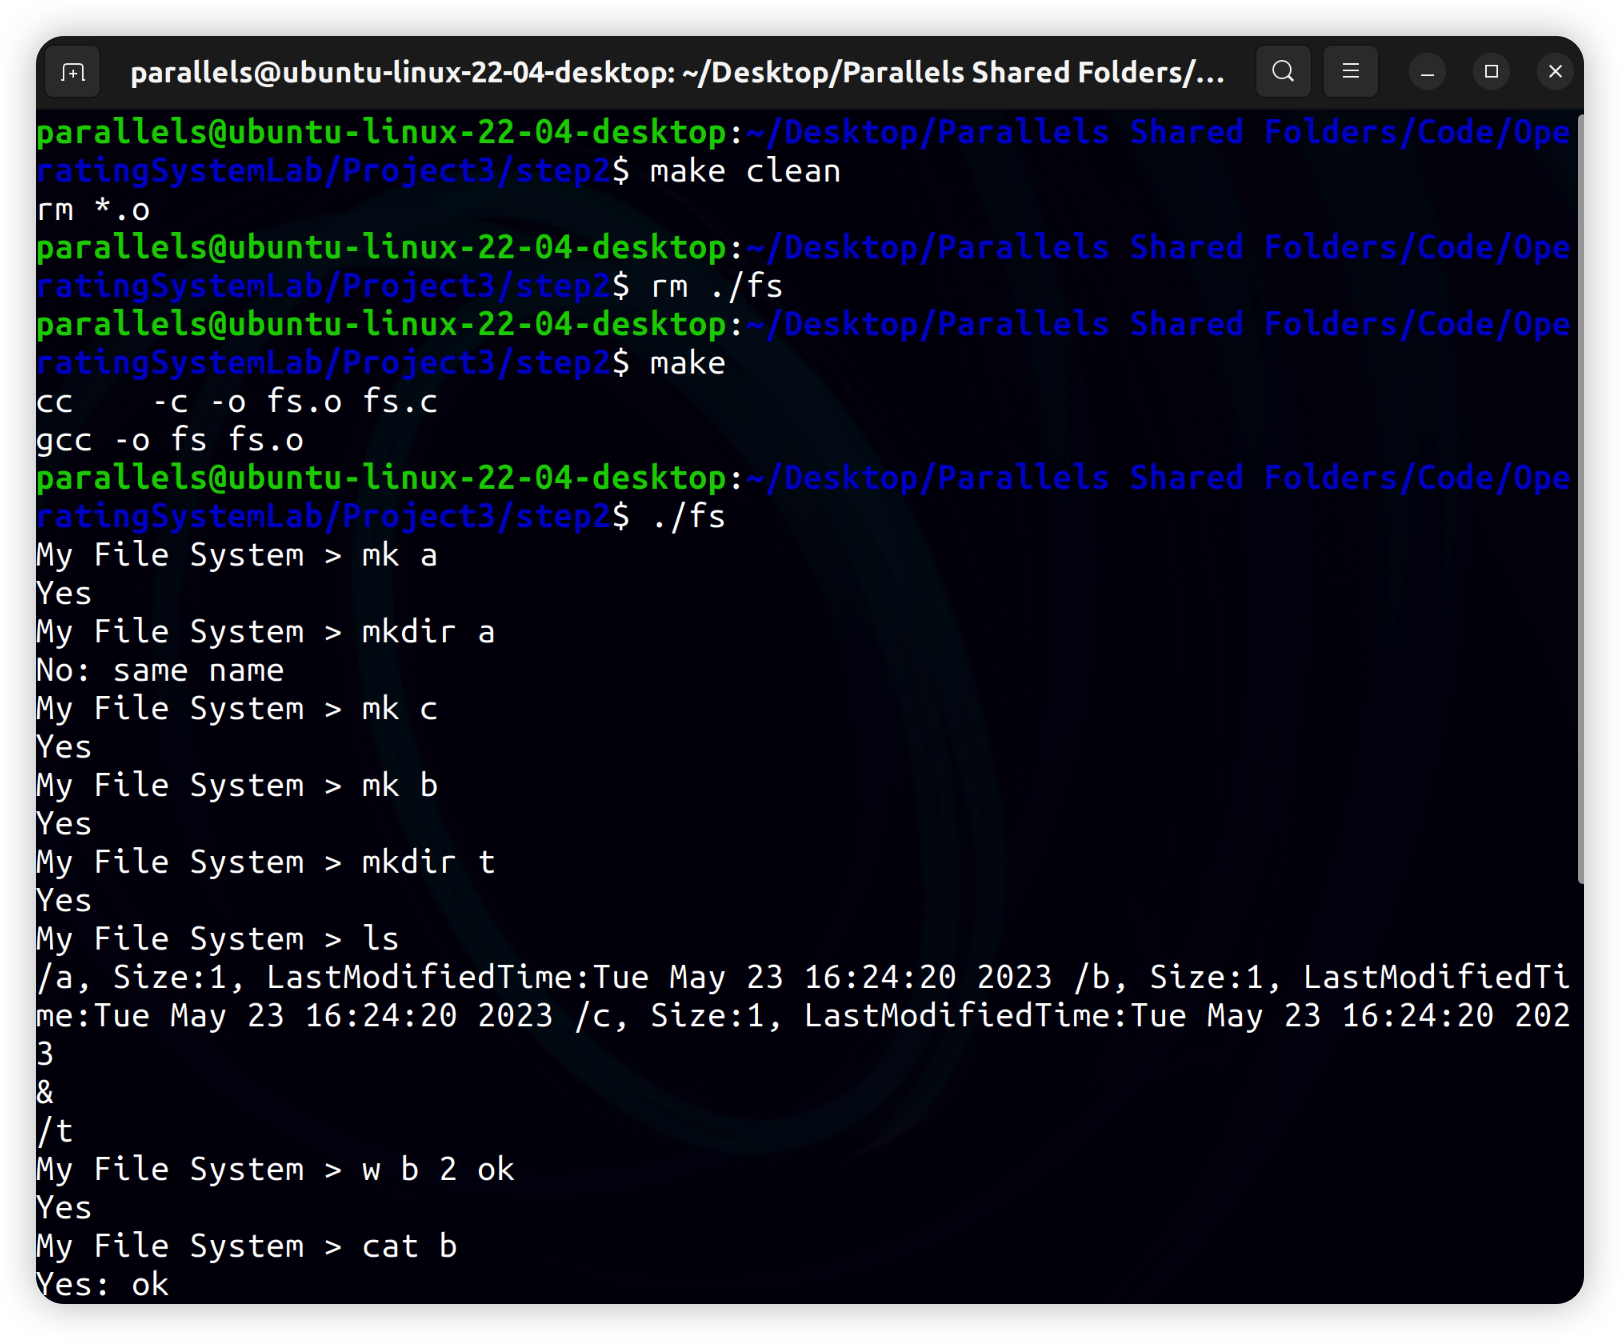
\includegraphics[scale = 0.35]{s2-t1.png}
\caption{Step2测试1}
\label{s2-t1}
\end{figure}

对指令 i f pos l data, d f pos l 进行了相应测试,输出符合要求。

\begin{figure}[H]
\center
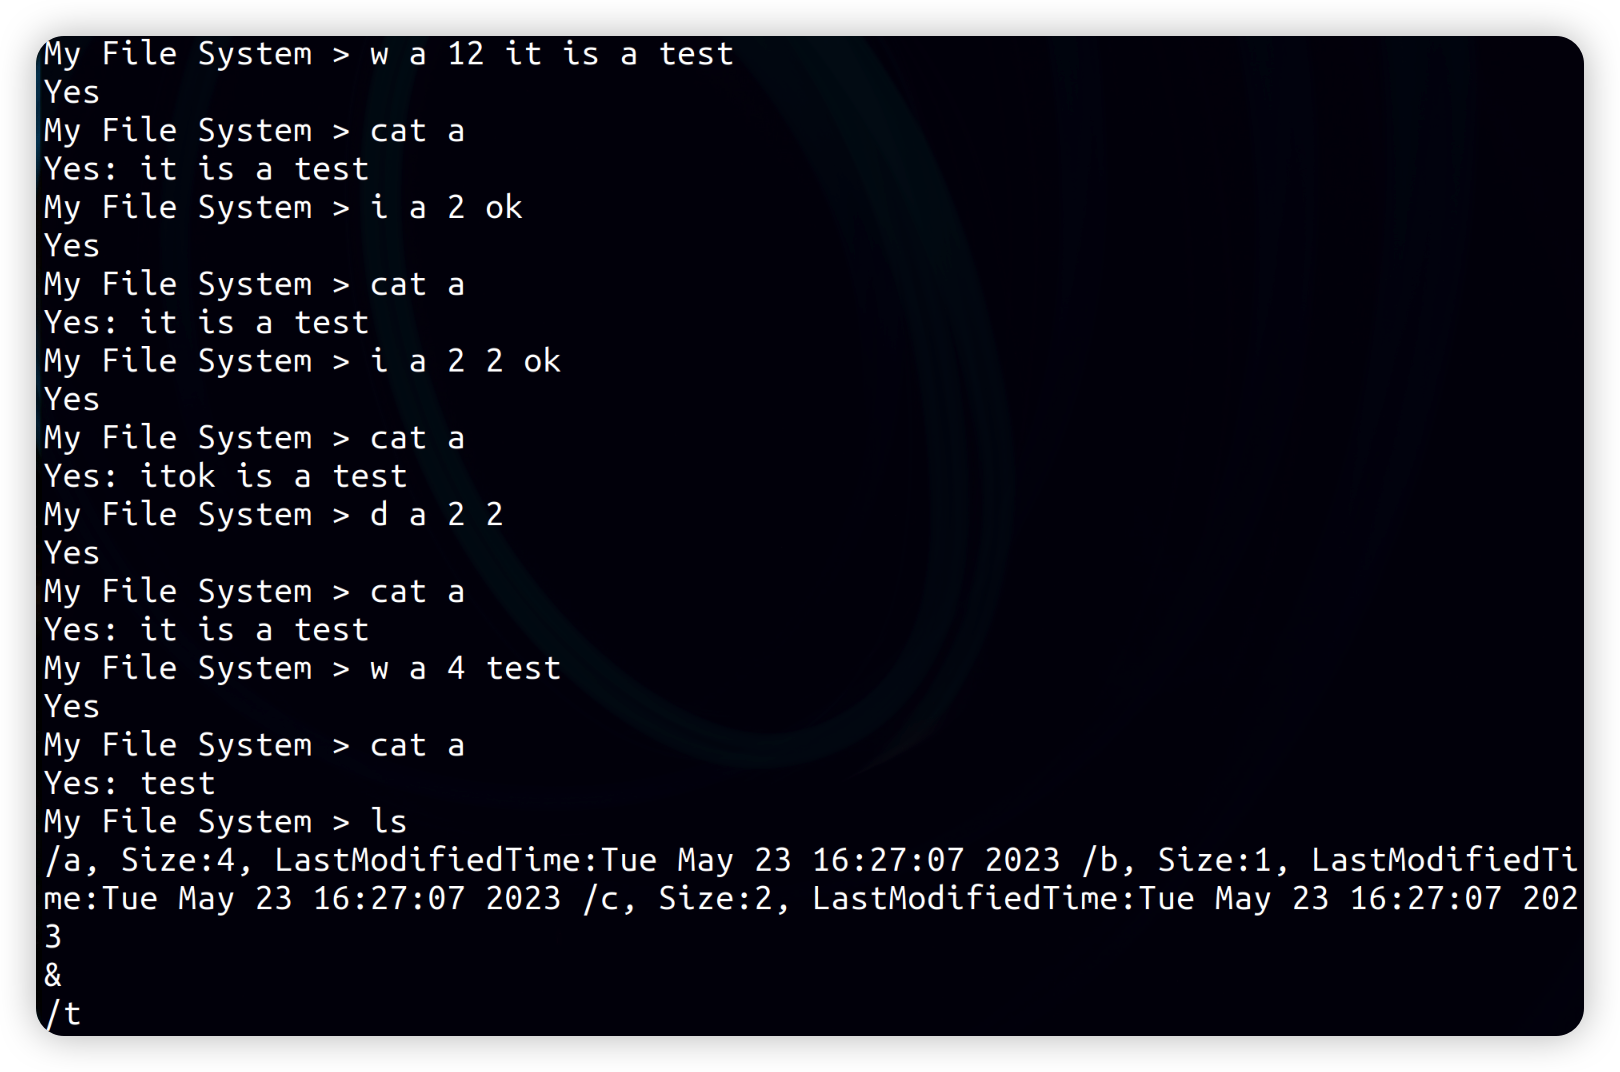
\includegraphics[scale = 0.35]{s2-t2.png}
\caption{Step2测试2}
\label{s2-t2}
\end{figure}

对指令 f ,e 进行了相应测试,输出符合要求。

\begin{figure}[H]
\center
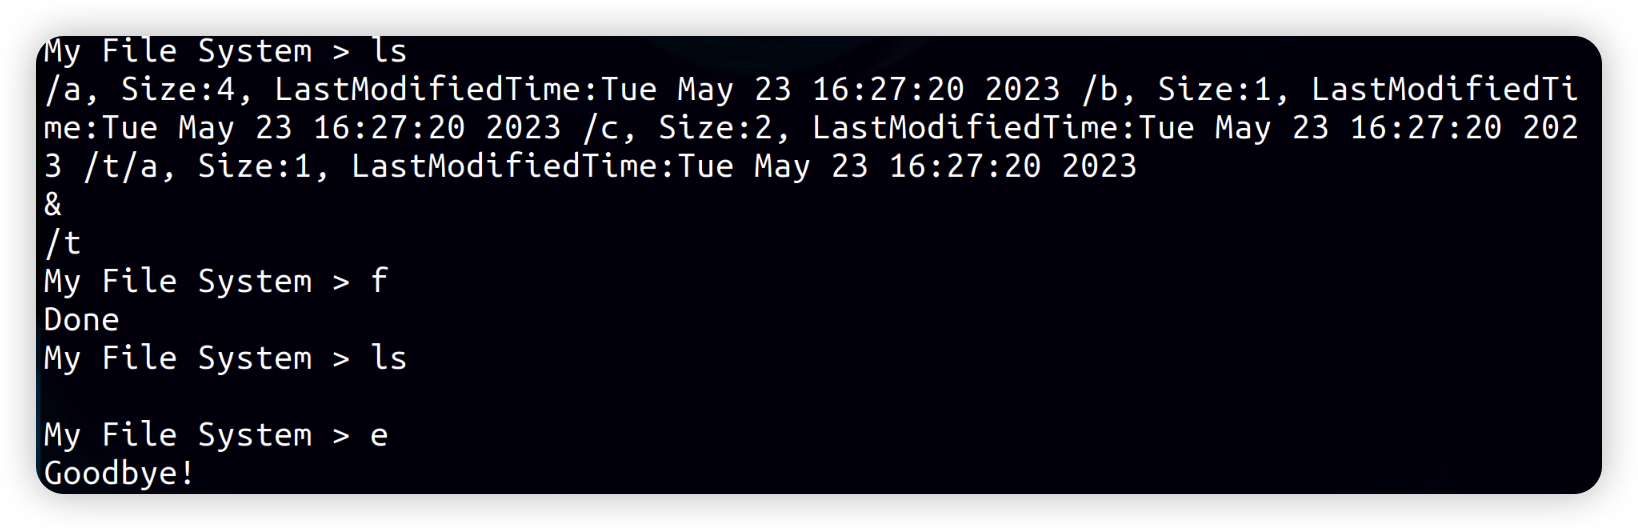
\includegraphics[scale = 0.35]{s2-t3.png}
\caption{Step2测试3}
\label{s2-t3}
\end{figure}

对指令 rm ,rmdir 进行了相应测试,输出符合要求。

\begin{figure}[H]
\center
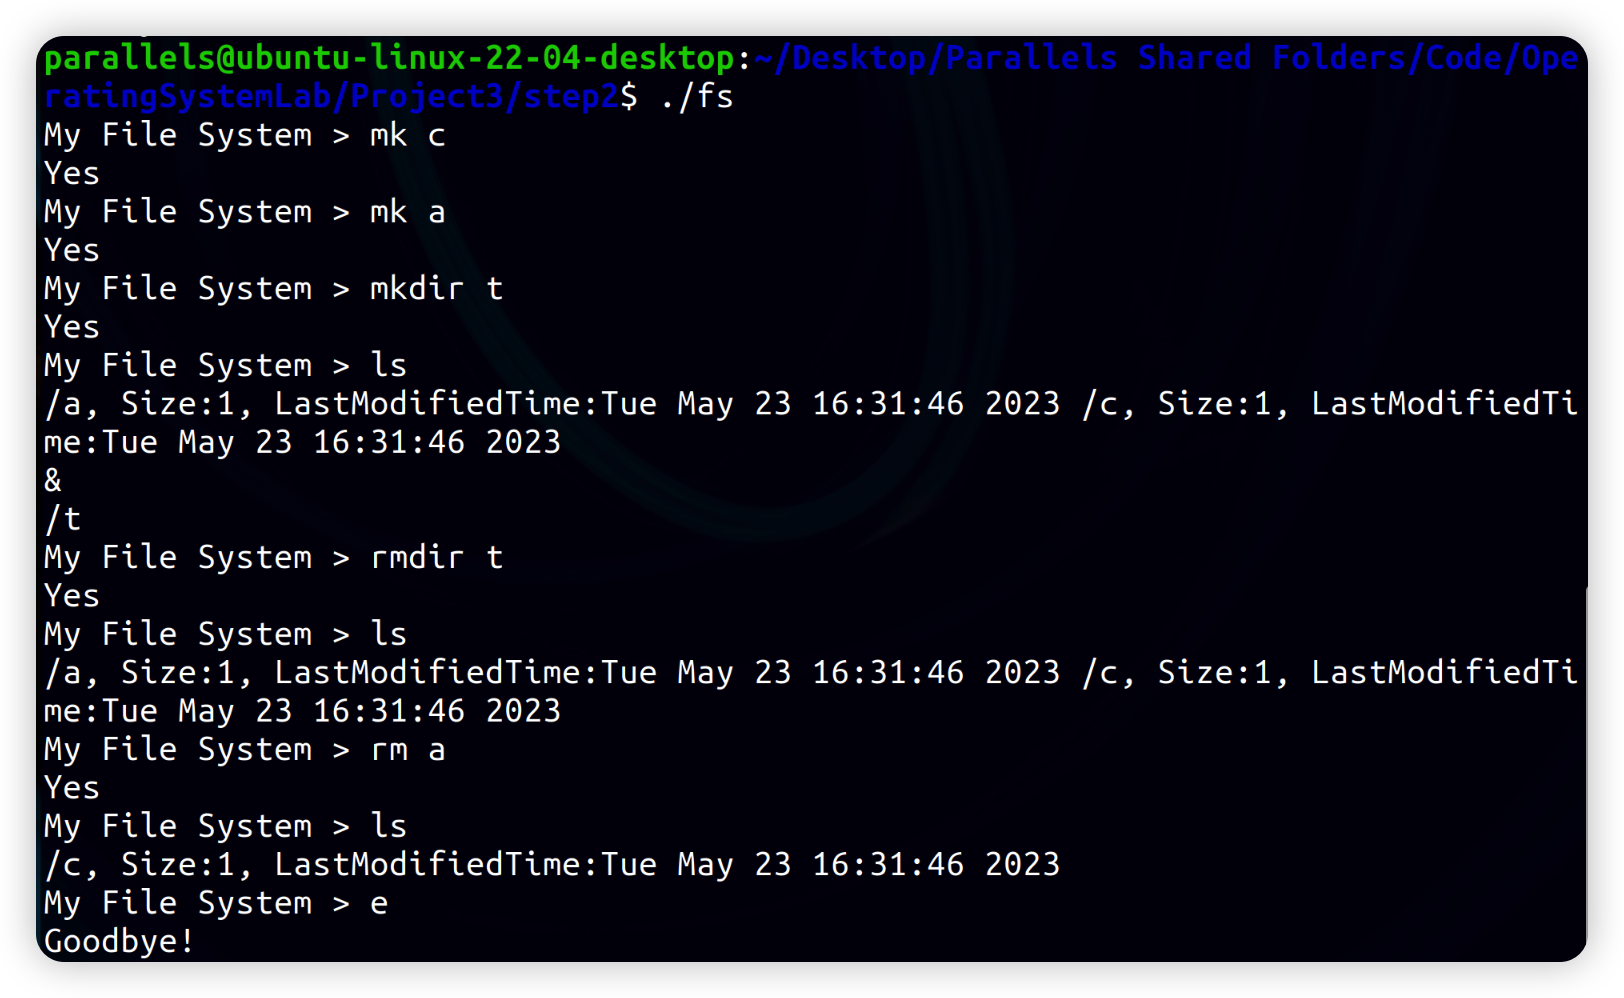
\includegraphics[scale = 0.35]{s2-t4.png}
\caption{Step2测试4}
\label{s2-t4}
\end{figure}

对指令 cd path ,cd., cd.. 进行了相应测试,输出符合要求。

\begin{figure}[H]
\center
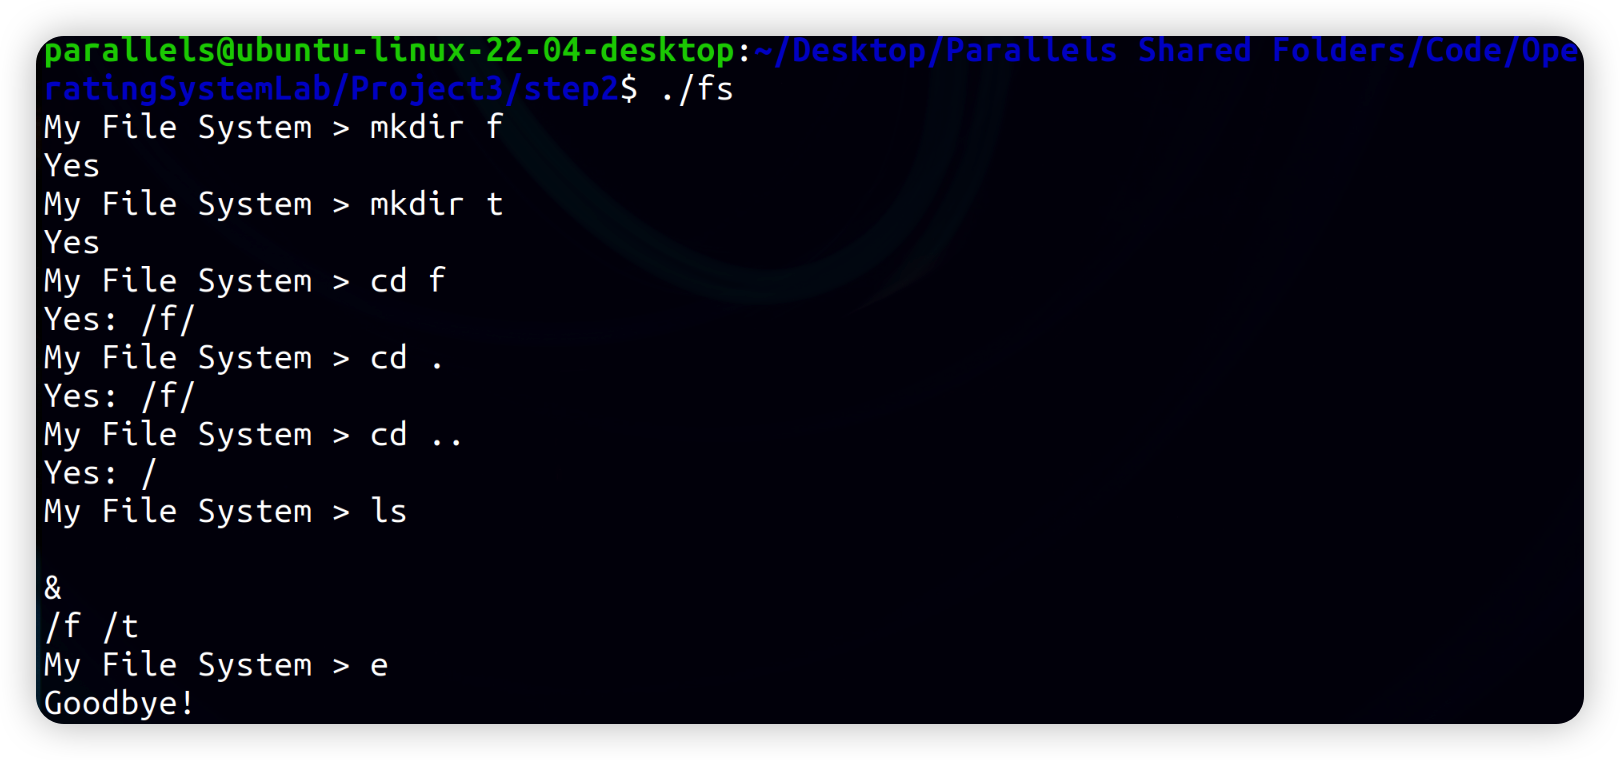
\includegraphics[scale = 0.35]{s2-t5.png}
\caption{Step2测试5}
\label{s2-t5}
\end{figure}

\section{Step3: Work together}

\subsection{实现要点}

\subsubsection{socket 结构构建}

与 Project1 类似,进行 Client 构建,修改其中读写顺序为 “写-读-写-读...” 使之与 fs 相匹配。

disk 作为服务器端,构建亦与 Project1 类似,这里不再赘述。修改其中读写顺序为  “读-写-读-写...”。

在 fs 文件中需要进行客户端和服务器的构建,使用两套 socket 构建。对客户端读写顺序为 “读-写-读-写...”,对 disk 端进行读写顺序为 “写-读-写-读...”。

\begin{lstlisting}
	// client part
    disk_portno = atoi(argv[2]);
    disk_sockfd = socket(AF_INET, SOCK_STREAM, 0);
    if (disk_sockfd < 0) 
        error("ERROR opening socket");
    disk_server = gethostbyname(argv[1]);
    if (disk_server == NULL) {
        fprintf(stderr,"ERROR, no such host\n");
        exit(0);
    }
    bzero((char *) &disk_serv_addr, sizeof(disk_serv_addr));
    disk_serv_addr.sin_family = AF_INET;
    bcopy((char *)disk_server->h_addr, 
         (char *)&disk_serv_addr.sin_addr.s_addr,
         disk_server->h_length);
    disk_serv_addr.sin_port = htons(disk_portno);
    if (connect(disk_sockfd,(struct sockaddr *) &disk_serv_addr,sizeof(disk_serv_addr)) < 0) 
        error("ERROR connecting");
    
    // server part
    sockfd = socket(AF_INET, SOCK_STREAM, 0);
    if (sockfd < 0) 
        error("Error opening socket");
    printf("Accepting connections ...\n");
    bzero((char *) &serv_addr, sizeof(serv_addr));
    portno = atoi(argv[3]);
    serv_addr.sin_family = AF_INET;
    serv_addr.sin_addr.s_addr = INADDR_ANY;
    serv_addr.sin_port = htons(portno);

    if (bind(sockfd, (struct sockaddr *) &serv_addr,sizeof(serv_addr)) < 0) 
        error("Error on binding");
    listen(sockfd,5);
\end{lstlisting}

用 dup2 将输出内容重定向到相应的客户端,并用 fprintf 维护日志的内容。

\begin{lstlisting}
		// redirect to client
        dup2(newsockfd, STDOUT_FILENO);
        ...
        // print to log
        fprintf(fd_log, "Receive from PORT(%d): %s", cli_addr.sin_port, buffer);
\end{lstlisting}

\subsubsection{虚拟磁盘与物理磁盘交互}

\begin{figure}[H]
\center
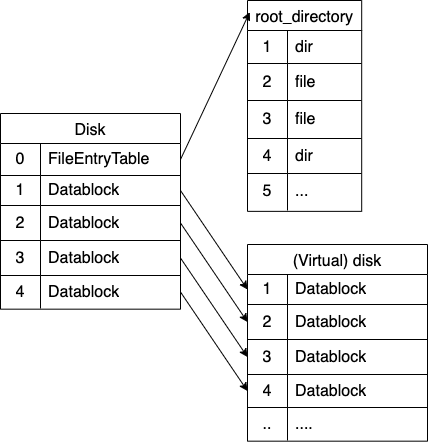
\includegraphics[scale = 0.6]{s3-1.png}
\caption{物理磁盘对应存储内容}
\label{s3-1}
\end{figure}

图\ref{s3-1}展示了虚拟 disk 与构建的服务端 disk 之间映射对应关系,其中第一个 block 存储 FileTable。受限于 block 大小,该文件系统一共支持至多 6 个文件(含目录)。

在创建文件,读文件,插入文件,删除内容,删除文件这些部分需要对虚拟 disk 进行读写,增加服务端 disk 后,用 R c s data 指令对相应数据块同步进行更新。

\begin{lstlisting}
...
			sprintf(disk_buffer, "W %d %d %s\n", root_directory[i].start_block/CYLINDERS, root_directory[i].start_block%CYLINDERS, disk[start_block]);
            disk_n = write(disk_sockfd, disk_buffer, strlen(disk_buffer));
            if (disk_n < 0) error("Error reading from socket");
            bzero(disk_buffer, 1024);
            disk_n = read(disk_sockfd, disk_buffer, 1023);
            if (disk_n < 0) error("Error reading from socket");
            printf("%s", disk_buffer);
            bzero(disk_buffer, 1024);
...
\end{lstlisting}

修改 disk.c 文件,增加对磁盘某一块的删除 D c s 操作和整体清空操作 C 以方便格式化文件系统操作和删除文件操作。并将写磁盘操作更改为在写之前重置磁盘内容。

\begin{lstlisting}
			else if (cmd == 'W') {
            // Write request
            sscanf(buf, "%d %d %[^\n]", &c, &s, instr);
            fprintf(fd_log, "command: W %d %d %s\n", c, s, instr);
            if (c < 0 || c >= CYLINDERS || s < 0 || s >= SECTORS) {
                printf("No\n");
            }
            else {
                strcpy(data, instr);
                memcpy(disk_data + (c * SECTORS + s) * BLOCKSIZE, data, strlen(data));
                printf("Yes\n");
                fprintf(fd_log, "Yes\n");
                usleep(track_to_track_time * abs(c - last_c));
            }
        }
        else if (cmd == 'D') {
            // Delete block
            sscanf(buf, "%d %d", &c, &s);
            fprintf(fd_log, "command: D %d %d\n", c, s);
            if (c < 0 || c >= CYLINDERS || s < 0 || s >= SECTORS) {
                printf("No\n");
            } 
            else {
                strcpy(data, "\0");
                memcpy(disk_data + (c * SECTORS + s) * BLOCKSIZE, data, 1);
                printf("Yes\n");
                fprintf(fd_log, "Yes\n");
                usleep(track_to_track_time * abs(c - last_c));
            }
        }
        else if (cmd == 'C') {
            fprintf(fd_log, "command: C\n");
            // Clear all
            for(int i = 0; i < CYLINDERS; i ++){
                for(int j = 0; j < SECTORS; j ++){
                    strcpy(data, "");
                    memcpy(disk_data + (i * SECTORS + j) * BLOCKSIZE, data, 1);
                }
            }
            printf("Yes\n");
            fprintf(fd_log, "Yes\n");
        }
\end{lstlisting}

\subsubsection{FileEntryTable 的存储}

DirectoryEntry 为一个结构体,在存入服务端 disk 的 block 块中需要先打包为字符串

\begin{lstlisting}
// pack DirectoryEntry in to a string
char* pack_dir(DirectoryEntry dir_entry) {
    char* packed_string = (char*)malloc(BLOCK_SIZE * sizeof(char));

    sprintf(packed_string, " %s %c %d %d %s|",
            dir_entry.filename, dir_entry.type, dir_entry.start_block, dir_entry.file_size, dir_entry.last_modified);
    return packed_string;
}
\end{lstlisting}

在此基础上,将整个 root\_directory 转化为字符串,并在开头添加 file\_count 以确定文件数量。

\begin{lstlisting}
void store_table() {
    char entry_table[BLOCK_SIZE] = "";
    if (file_count != 0){
        sprintf(entry_table, "%d", file_count);
        for(int i = 0; i < MAX_FILE_ENTRIES; i++){
            if(strcmp(root_directory[i].filename , "\0") == 0) continue;
            strncat(entry_table, pack_dir(root_directory[i]), strlen(pack_dir(root_directory[i])));
        }
        sprintf(disk_buffer, "W %d %d %s\n", 0, 0, entry_table);
        disk_n = write(disk_sockfd, disk_buffer, strlen(disk_buffer));
        if (disk_n < 0) error("Error reading from socket");
    }
    else{
        sprintf(disk_buffer, "C\n");
        disk_n = write(disk_sockfd, disk_buffer, strlen(disk_buffer));
        if (disk_n < 0) error("Error reading from socket");
    }
}
\end{lstlisting}

此函数在退出时调用,将最新的 FileEntryTable 存入物理磁盘中。

\subsubsection{FileSystem 的初始化}

在文件系统开始时需要获取磁盘信息以得知存储大小信息;利用上一次存入的 FileEntryTable 初始化目录表,并将数据块读入虚拟磁盘从而形成非易失的文件系统。

\begin{lstlisting}
	// initial CYLINDERS and SECTORS
    strcpy(disk_buffer, "I\n");
    disk_n = write(disk_sockfd, disk_buffer, strlen(disk_buffer));
    if (disk_n < 0) error("Error writing to socket");
    disk_n = read(disk_sockfd, disk_buffer, 1024);
    if (disk_n < 0) error("Error reading from socket");
    sscanf(disk_buffer, "%d %d", &CYLINDERS, &SECTORS);
    bzero(disk_buffer, 1024);

    // initial file allocation table
    sprintf(disk_buffer, "R %d %d\n", 0, 0);
    disk_n = write(disk_sockfd, disk_buffer, strlen(disk_buffer));
    if (disk_n < 0) error("Error writing to socket");
    disk_n = read(disk_sockfd, disk_buffer, 1024);
    if (disk_n < 0) error("Error reading from socket");
    unpack_dir(getValidString(disk_buffer), root_directory);
    bzero(disk_buffer, 1024);

    // initial virtual disk
    for(int i = 1; i < CYLINDERS * SECTORS; i++){
        sprintf(disk_buffer, "R %d %d\n", i/CYLINDERS, i%CYLINDERS);
        disk_n = write(disk_sockfd, disk_buffer, strlen(disk_buffer));
        if (disk_n < 0) error("Error reading from socket");
        bzero(disk_buffer, 1024);
        disk_n = read(disk_sockfd, disk_buffer, 1023);
        if (disk_n < 0) error("Error reading from socket");
        if(disk_buffer[0] == '\n') disk_buffer[0] = '\0';
        strncpy(disk[i], disk_buffer, BLOCK_SIZE);
        bzero(disk_buffer, 1024);
    }
\end{lstlisting}

在读取目录表时用到解析函数 unpack\_dir 函数,将字符串信息恢复成结构体数组。由于每一项在打包时用|进行分隔,在解析时可以使用 strchr 定位下一项内容。

\begin{lstlisting}
// Parse the struct from the string
void unpack_dir(const char* packed_string, DirectoryEntry* dir_entry) {
    if(strcmp(packed_string, "\0") == 0){
        file_count = 0;
        return;
    }
    sscanf(packed_string, "%d", &file_count);
    const char* current_position = packed_string + 1;

    for (int i = 0; i < file_count; i++) {
        sscanf(current_position, " %s %c %d %d %[^|]",
            dir_entry[i].filename, &dir_entry[i].type, &dir_entry[i].start_block, &dir_entry[i].file_size, dir_entry[i].last_modified);
        
        // Navigate to the location of the next directory entry
        current_position = strchr(current_position, '|');
        if (current_position == NULL) {
            printf("Invalid packed_string format\n");
            return;
        }
        current_position++; // Jump '|'
    }
}
\end{lstlisting}

\subsection{功能测试}

\subsubsection{基础功能测试}

由于 Step2 进行了完善的测试,这里进行简单的测试,相应内容符合要求。

\begin{figure}[H]
\center
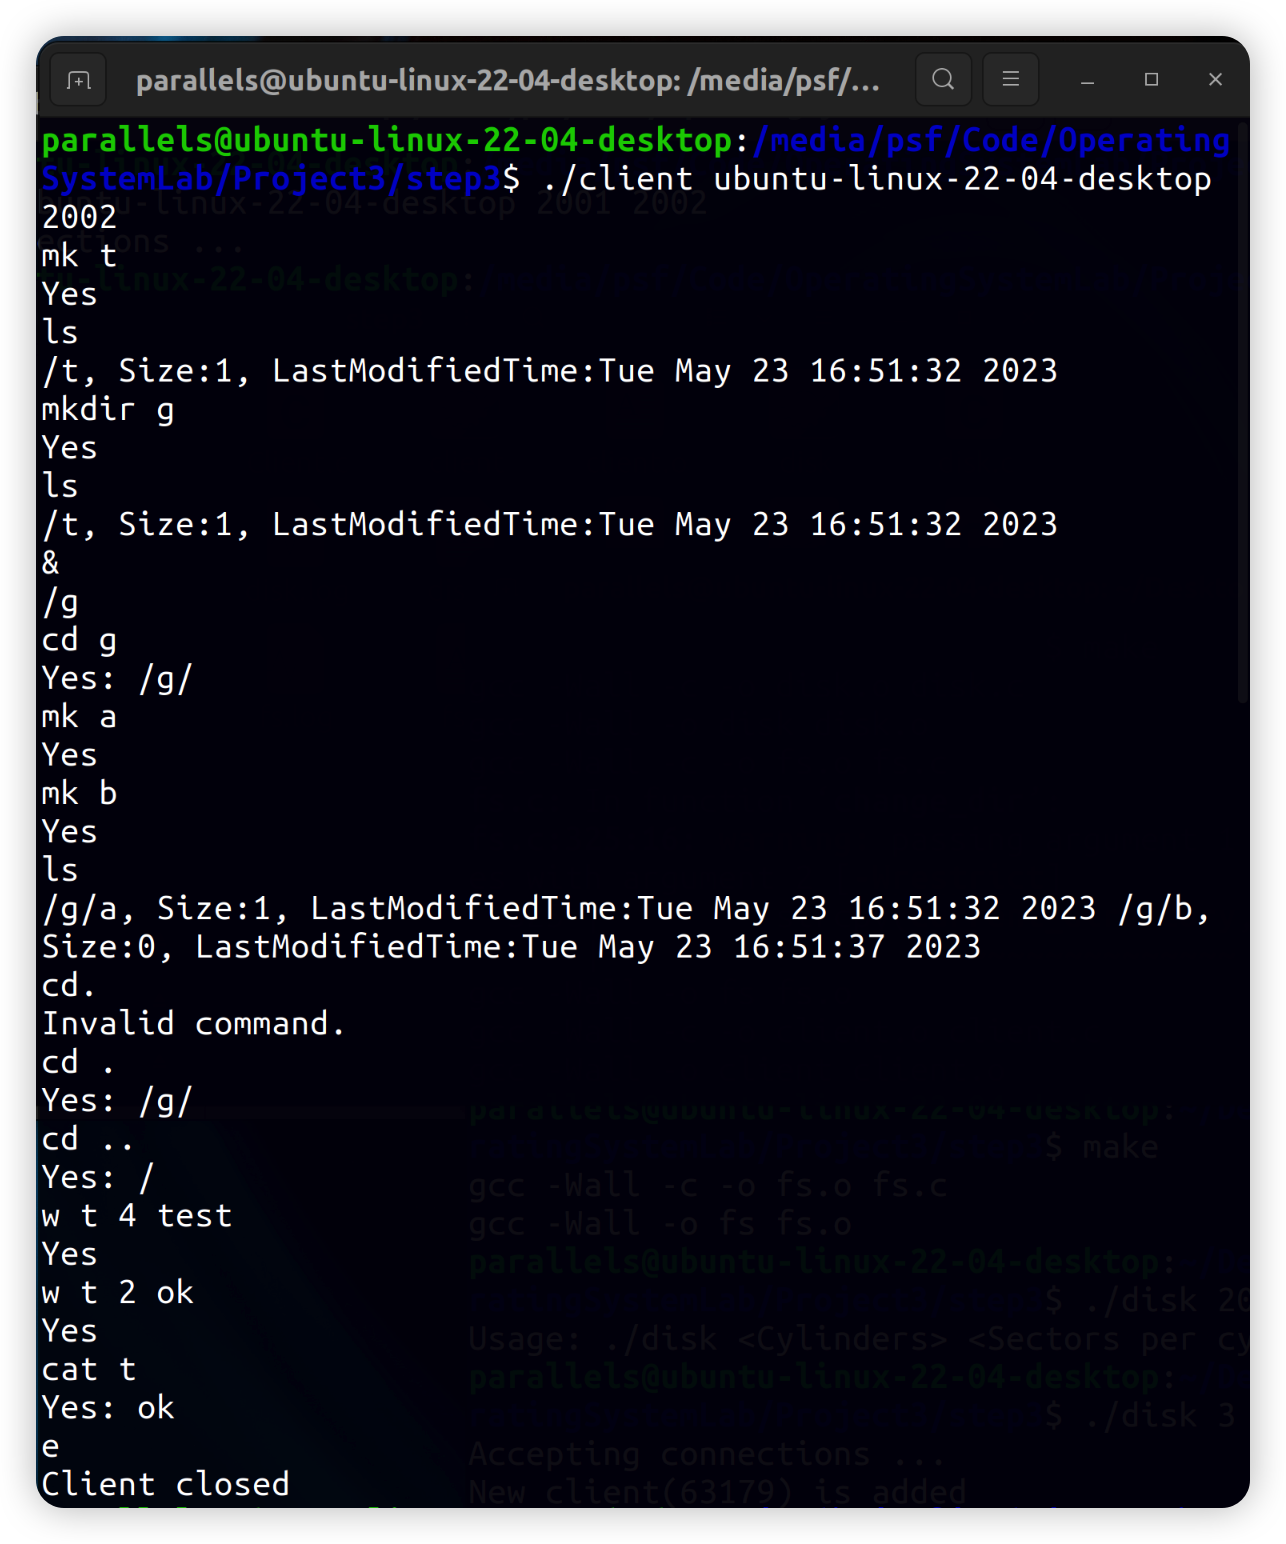
\includegraphics[scale = 0.5]{s3-t1.png}
\caption{Step3测试1}
\label{s3-t1}
\end{figure}

所维护的两个日志文件内容如图\ref{s3-t2}\ref{s3-t3}所示。

\begin{figure}[H]
\center
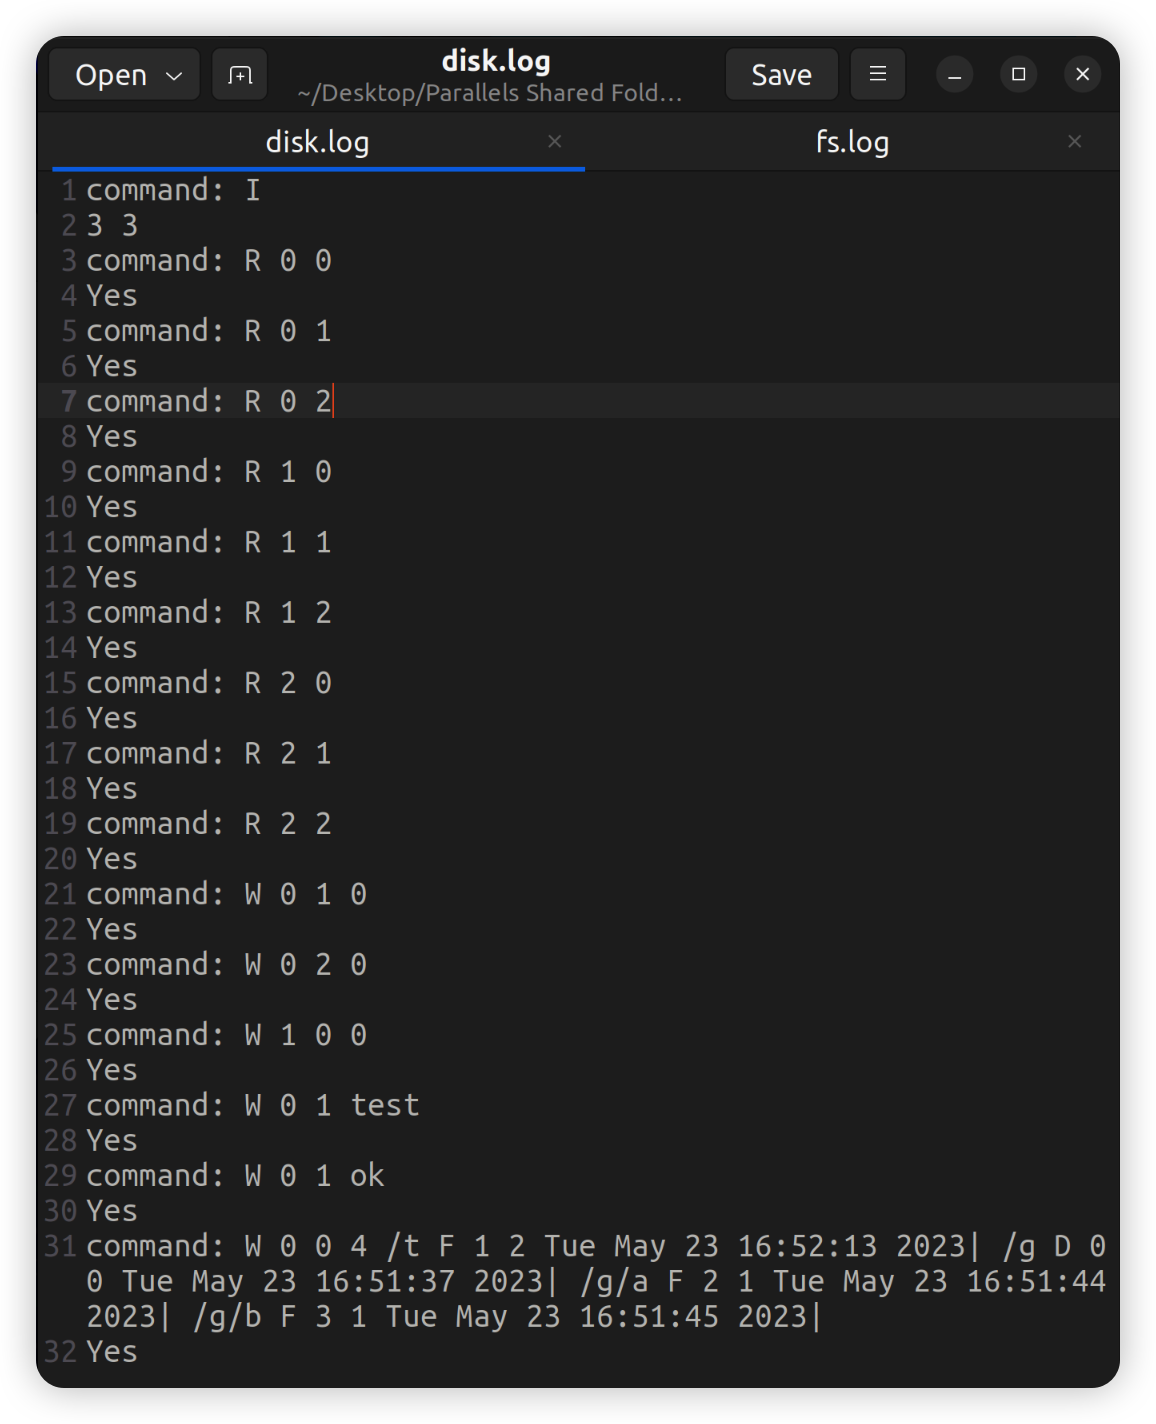
\includegraphics[scale = 0.4]{s3-t2.png}
\caption{disk.log内容}
\label{s3-t2}
\end{figure}

\begin{figure}[H]
\center
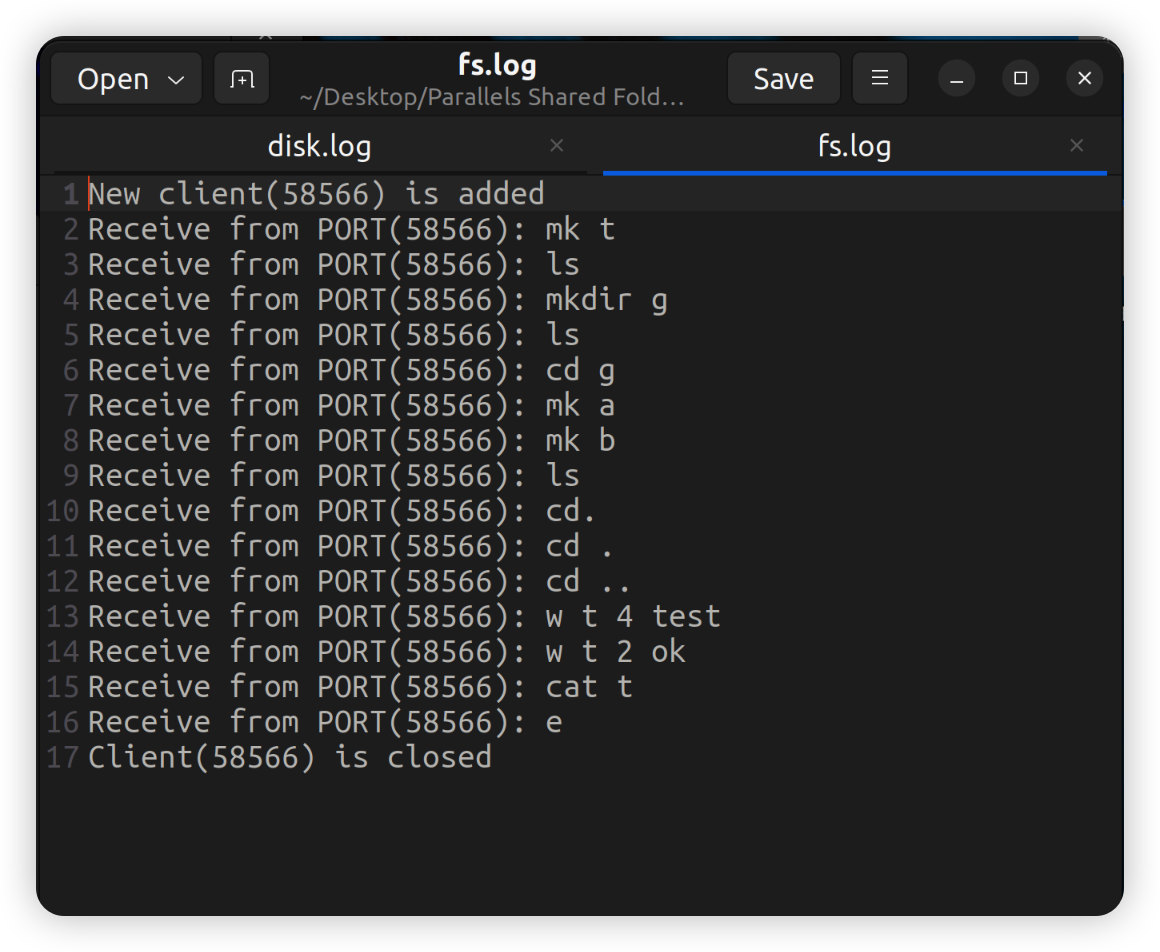
\includegraphics[scale = 0.4]{s3-t3.png}
\caption{fs.log内容}
\label{s3-t3}
\end{figure}

\subsubsection{恢复功能测试}

在进行联合后,文件系统拥有非易失特性,可从上一次的系统情况继续操作,测试结果如图\ref{s3-t4}。

\begin{figure}[H]
\center
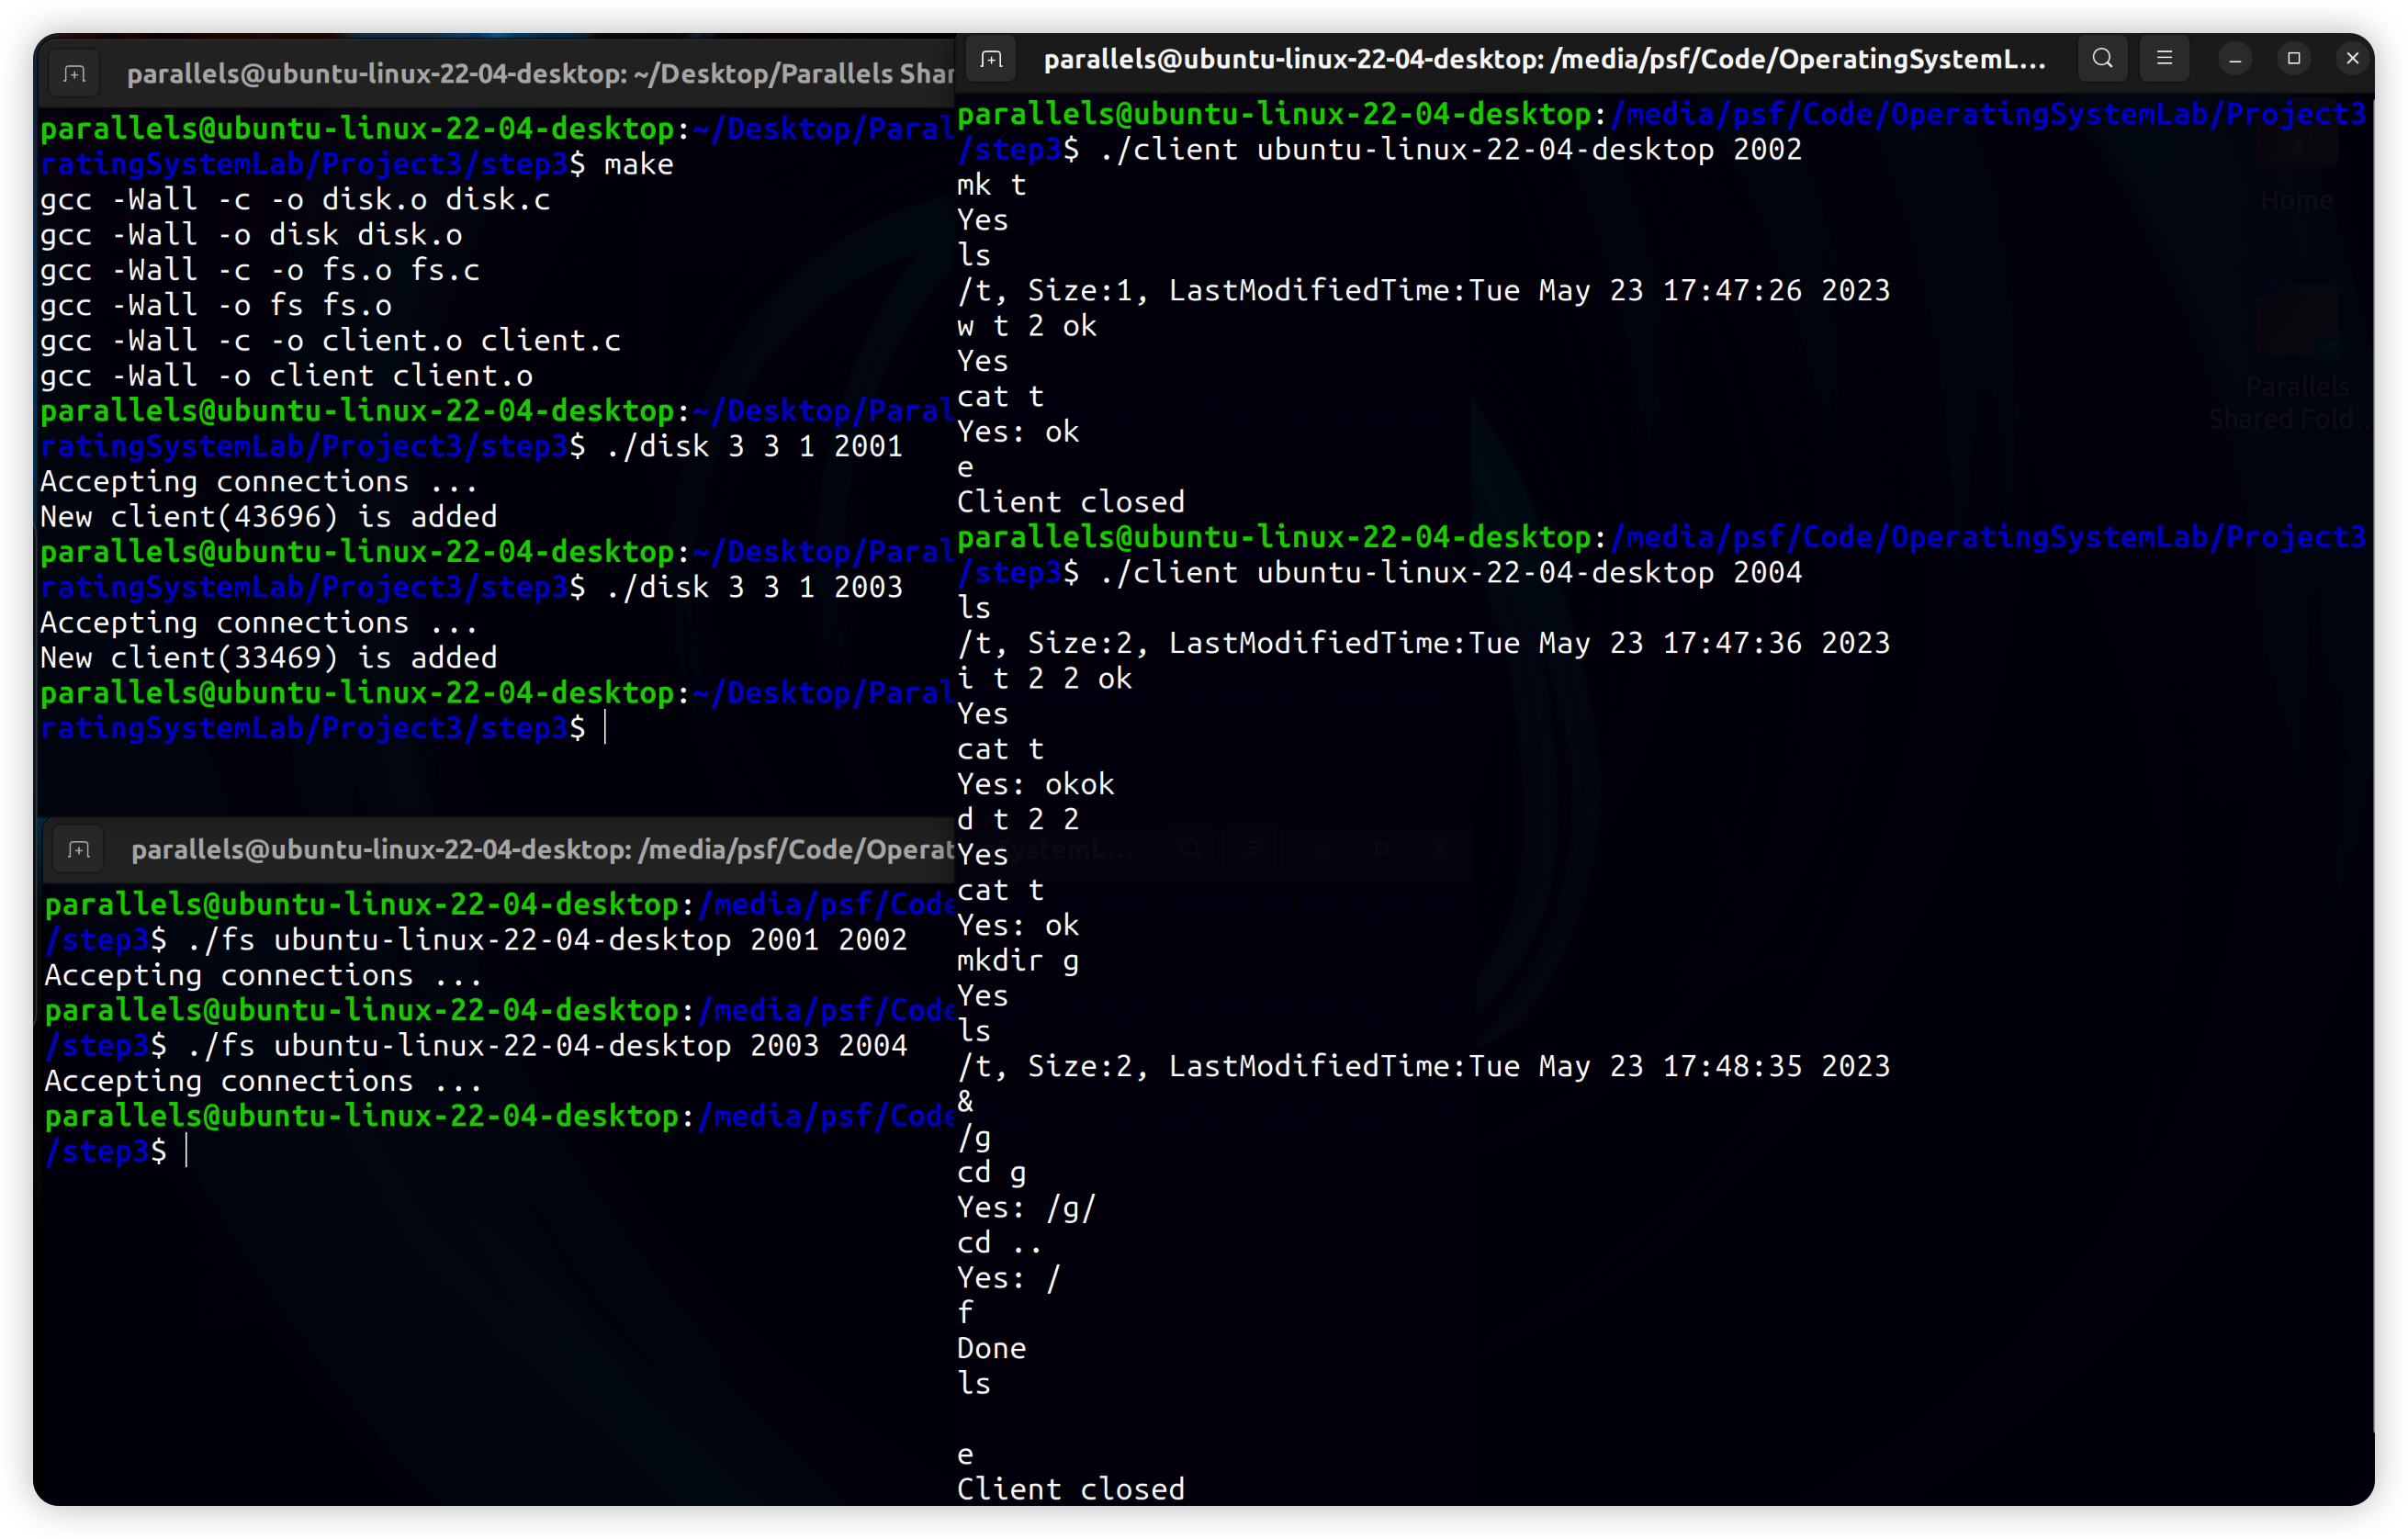
\includegraphics[scale = 0.3]{s3-t4.png}
\caption{恢复功能测试}
\label{s3-t4}
\end{figure}

\newpage
\section*{总结与反思}
\addcontentsline{toc}{section}{总结与反思}
\setlength{\parindent}{2em}

本次实验首先设计和实现了一个基本的类似磁盘的辅助存储服务器;接着实现了一个基本的 FAT 结构文件系统;在此基础上用磁盘当服务器,用 socket 套接字使得文件系统能够和磁盘服务器交互写作,形成一个非易失文件系统,并将其作为第二级服务器,用客户端连接访问。 并在 linux 系统上进行了测试,证明了该文件系统基本实现了相关要求。

由于多服务端端特性,调试过程困难繁琐。在此总结实验过程中的易错问题及其解决:

\begin{itemize}
	\item buffer 以换行符作为一次读取的标准,需要在输出时谨慎,例如 ctime 转换的字符串末尾会带上换行符。
	\item 由于服务器和客户端采用阻塞读写,双方需协调好读写顺序,若出现多读,多写与少读,少写的情况会导致整个系统卡死。
	\item 日志文件采用 int fd\_log = open("disk.log", O\_WRONLY | O\_CREAT, S\_IRUSR | S\_IWUSR); 的方式打开操作繁琐且会出现乱码的情况,读写情况不透明。后期改为 File* fd\_log = fopen("fs.log", "w"); 的方式创建文件。
	\item disk 并不真正“删除”某些数据,通过在开头添加\verb |\0| 作为格式化方案。
\end{itemize}

本次实验使我对文件系统特性的了解大大加深,也大大提高我 c 语言处理内存,字符串和调试的能力。

该文件系统仍然存在不少不足的地方:

\begin{itemize}
	\item 采用的 FAT 结构相较于 I-node 在效率上和拓展性上存在不足。
	\item 支持的文件数量较少且文件大小有限制,拓展性能不足。
	\item 未对输出进行进一步的美化工作,较为简陋。
	\item 文件的写入不支持回车等特殊情况。
\end{itemize}

总之,这是一个微型的文件系统,能够在一定程度上实现功能,却仍有很大进步空间。

\end{document}




